\begin{figure}[h]
    \centering
    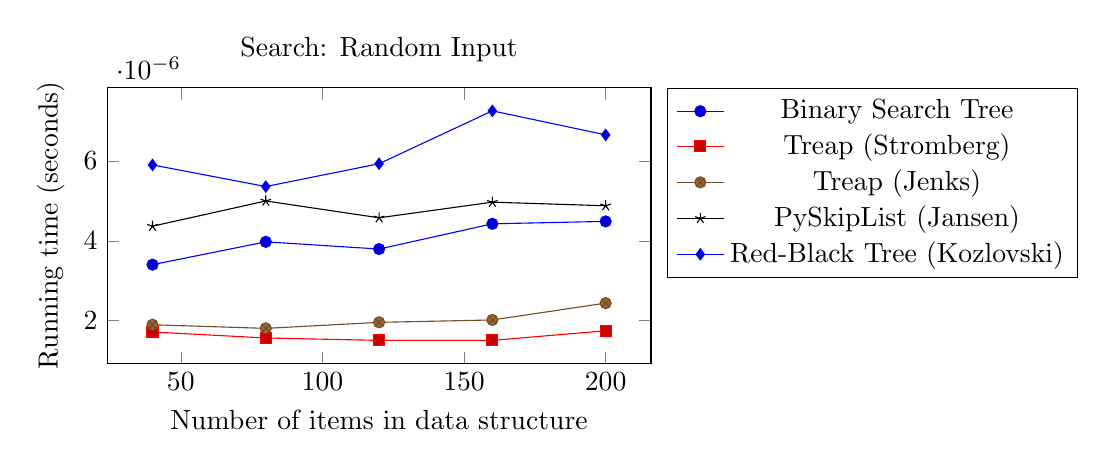
\begin{tikzpicture}
        \begin{axis}[
            xlabel={Number of items in data structure},
            ylabel={Running time (seconds)},
            title={Search: Random Input},
            width=0.7\textwidth,
            height=2in,
            legend pos=outer north east
        ]
		\addplot coordinates {
			(40, 3.403281305293382e-06)
			(80, 3.975514445122424e-06)
			(120, 3.7948092430711845e-06)
			(160, 4.4272774502494835e-06)
			(200, 4.487512517600128e-06)
		};
		\addplot coordinates {
			(40, 1.7166994194843522e-06)
			(80, 1.5661117511084343e-06)
			(120, 1.5058766837584836e-06)
			(160, 1.5058766837584836e-06)
			(200, 1.7468169531596745e-06)
		};
		\addplot coordinates {
			(40, 1.8974046215355922e-06)
			(80, 1.8070520205103192e-06)
			(120, 1.9576396888862367e-06)
			(160, 2.0178747562361876e-06)
			(200, 2.4395202276886186e-06)
		};
		\addplot coordinates {
			(40, 4.367042382899533e-06)
			(80, 4.999510590077833e-06)
			(120, 4.577865118625401e-06)
			(160, 4.9693930564025105e-06)
			(200, 4.879040455377237e-06)
		};
		\addplot coordinates {
			(40, 5.903036600332645e-06)
			(80, 5.360920994179619e-06)
			(120, 5.933154134007967e-06)
			(160, 7.258325615715211e-06)
			(200, 6.655974942212927e-06)
		};
        \legend{Binary Search Tree, Treap (Stromberg), Treap (Jenks), PySkipList (Jansen), Red-Black Tree (Kozlovski)}
        \end{axis}
    \end{tikzpicture}
    \caption{Average of 10 operations, benchmarked every 40, starting at 40.}
\end{figure}